%
% The first command in your LaTeX source must be the \documentclass command.
\documentclass[sigchi]{acmart}

%
% defining the \BibTeX command - from Oren Patashnik's original BibTeX documentation.
\def\BibTeX{{\rm B\kern-.05em{\sc i\kern-.025em b}\kern-.08emT\kern-.1667em\lower.7ex\hbox{E}\kern-.125emX}}

    
% Rights management information. 
% This information is sent to you when you complete the rights form.
% These commands have SAMPLE values in them; it is your responsibility as an author to replace
% the commands and values with those provided to you when you complete the rights form.
%
% These commands are for a PROCEEDINGS abstract or paper.
\copyrightyear{2025}
\acmYear{2025}
\setcopyright{acmlicensed}
\acmConference[SNA '24]{Social Network Analysis '24}{2023/24}{University of Pisa, Italy}
\acmBooktitle{Social Network Analysis '24}
\acmPrice{0.00}
%\acmDOI{10.1145/1122445.1122456}
%\acmISBN{978-1-4503-9999-9/18/06}


% end of the preamble, start of the body of the document source.
\begin{document}

%
% The "title" command has an optional parameter, allowing the author to define a "short title" to be used in page headers.
\title{Diffusione delle Opinioni Politiche e Dinamiche di Community su Reddit}

%costruzione
% The "author" command and its associated commands are used to define the authors and their affiliations.
% Of note is the shared affiliation of the first two authors, and the "authornote" and "authornotemark" commands
% used to denote shared contribution to the research.
\author{Caridi Leonardo}
\email{l.caridi@studenti.unipi.it}
\affiliation{%
  \institution{Student ID: 578938}
}


%\renewcommand{\shortauthors}{One and Two, et al.}


% The abstract is a short summary of the work to be presented in the article.
\begin{abstract}
Il 13 luglio 2024, in Pennsylvania, si verifica un attentato contro Donald Trump. Circa una settimana dopo, il 21 luglio 2024, Kamala Harris annuncia ufficialmente la sua candidatura alle primarie democratiche. Questo report analizza le reazioni di alcuni utenti di Reddit a questi eventi, prima attraverso un modello di diffusione delle opinioni e successivamente con un modello di dinamica delle community.

\footnote{
{\bf Project Repositories}\\
\noindent Data Collection: \url{https://github.com/LeonardoCaridi/2024_caridi/tree/main/data_collection}\\
\noindent Analytical Tasks: \url{https://github.com/LeonardoCaridi/2024_caridi/tree/main/network_analysis}\\
\noindent Report: \url{https://github.com/LeonardoCaridi/2024_caridi/tree/main/report}}
\end{abstract}


%
% Keywords. The author(s) should pick words that accurately describe the work being
% presented. Separate the keywords with commas.
\keywords{Social Network Analysis, Opinion Dynamics, Dynamic Community Discovery, politics}


%
% This command processes the author and affiliation and title information and builds
% the first part of the formatted document.
\maketitle

\section{Introduzione} \label{sec:introduction}
Come si diffonde l'opinione degli utenti di Reddit in risposta a eventi politici di grande impatto? Come si trasformano le community nel tempo? Questo report esplora queste dinamiche analizzando due eventi cruciali per le elezioni statunitensi del 2024: l'attentato a Donald Trump il 13 luglio e la candidatura di Kamala Harris il 21 luglio.

L'effetto del secondo evento è riuscito a contrastare le reazioni generate dal primo? La candidatura di Harris ha attenuato la discussione scatenata dall'attentato? Per rispondere, il comportamento degli utenti viene studiato su un periodo di sei settimane, con il 13 luglio come punto centrale. In questa scala temporale, l'attentato segna l'inizio della quarta settimana, mentre la candidatura di Harris si colloca nel secondo giorno della quinta.

Nella Sezione \ref{sec:data_collection} vengono esposti i metodi di raccolta, costruzione e semplificazione del grafo. Nella Sezione \ref{sec:network_characterization} vengono analizzate le principali caratteristiche del grafo, confrontandole con modelli sintetici come il random graph, lo small world graph e lo scale-free graph. Nella Sezione \ref{sec:diffusion_opinion} viene sviluppato un modello per simulare la diffusione delle opinioni all'interno del network. Successivamente, nella Sezione \ref{sec:evoluzione_community} il grafo viene diviso in sei snapshot (uno per ogni settimana) per studiare l'evoluzione delle community con un modello instant optimal. Infine, nella Sezione \ref{sec:conclusioni} vengono discussi i risultati e proposte delle possibili modifiche all'analisi.

\section{Data Collection} \label{sec:data_collection}
Grazie al tool \href{https://arctic-shift.photon-reddit.com/download-tool}{Project Arctic Shift} di \href{https://github.com/ArthurHeitmann/arctic_shift.git}{Arthur Heitmann}, è stato possibile scaricare post e commenti specificando i subreddit di interesse e l'intervallo temporale. I subreddit selezionati sono \textit{r/trump}, \textit{r/Conservative}, \textit{r/democrats}, \textit{r/KamalaHarris}, \textit{r/JoeBiden} e \textit{r/Liberal}. Per garantire il bilanciamento delle fonti, i subreddit pro-Biden sono stati scelti in numero doppio rispetto a quelli pro-Trump, ottenendo una distribuzione approssimativa del $\sim60\%$ pro-Trump e $\sim40\%$ pro-Biden (come si vede nella legenda di Figura \ref{fig:gephi_graph}). 

Il grafo è stato costruito rappresentando gli utenti come nodi e i commenti come archi direzionali, con un peso proporzionale al numero di interazioni tra i due utenti. Sono stati successivamente rimossi gli utenti eliminati, i self-loop, gli utenti il cui nome contiene la parola 'bot' e i moderatori, selezionati manualmente. Dopo questi passaggi, il grafo conta circa $\sim 60k$ nodi e $\sim 294k$ archi. Per semplificare ulteriormente, sono stati esclusi gli utenti con una sola interazione, riducendo il grafo a circa $\sim 37k$ nodi e $\sim 267k$ archi.

\subsection{Backboning}
Per ridurre ulteriormente la complessità del grafo, è stato applicato un metodo di backboning, in particolare il \textit{disparity filter}. Questo metodo seleziona gli archi più rilevanti confrontando i pesi con un modello di ipotesi nulla che estrae i pesi in modo uniforme. Se l'arco ha un p-value superiore a un valore critico (ad esempio 0.05), viene scartato. Il modello è stato implementato tramite il file \href{https://github.com/sna-unipi/ANC-lectures-notebooks/blob/main/backboning.py}{\textit{backboning}}, fornito nella cartella \href{https://github.com/sna-unipi/ANC-lectures-notebooks}{\textit{ANC-lectures-notebooks}}. In questo caso, invece del p-value, il file utilizza il valore complementare \texttt{score}, e la selezione degli archi avviene confrontando lo \texttt{score} con una soglia (threshold). Gli archi con uno \texttt{score} inferiore alla soglia vengono scartati. Per mantenere il numero di nodi sopra il limite minimo consentito ($10k-15k$), è stata impostata una threshold di $0.6$, ottenendo un grafo finale con circa $\sim19k$ nodi e $\sim73k$ archi.

Nella Figura \ref{fig:backboning_dist} si osserva che le forme delle distribuzioni non mostrano cambiamenti sostanziali rispetto al grafo precedente al backboning. Tuttavia, è evidente una diminuzione dei degree dei nodi e del global cluster coefficient, causata dalla riduzione del numero di nodi e archi. In particolare, l'average degree passa da circa $\sim 14$ a $\sim 7$, mentre il global clustering diminuisce da circa $\sim 0.082$ a $\sim 0.023$. Questi risultati sono attesi, dato che il numero di nodi è stato ridotto di circa la metà e il numero di archi è diminuito di circa un quarto rispetto alla versione precedente del grafo.

\begin{figure}[h]
    \centering
    \begin{minipage}{0.48\textwidth}
        \centering
        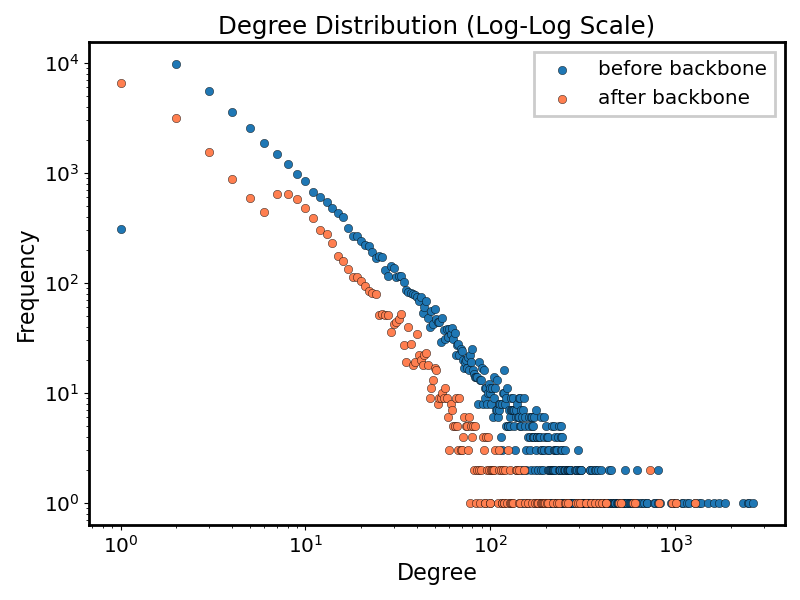
\includegraphics[width=\linewidth]{img/Degree Distribution (Log-Log Scale).png}
    \end{minipage}
    \hfill
    \begin{minipage}{0.48\textwidth}
        \centering
        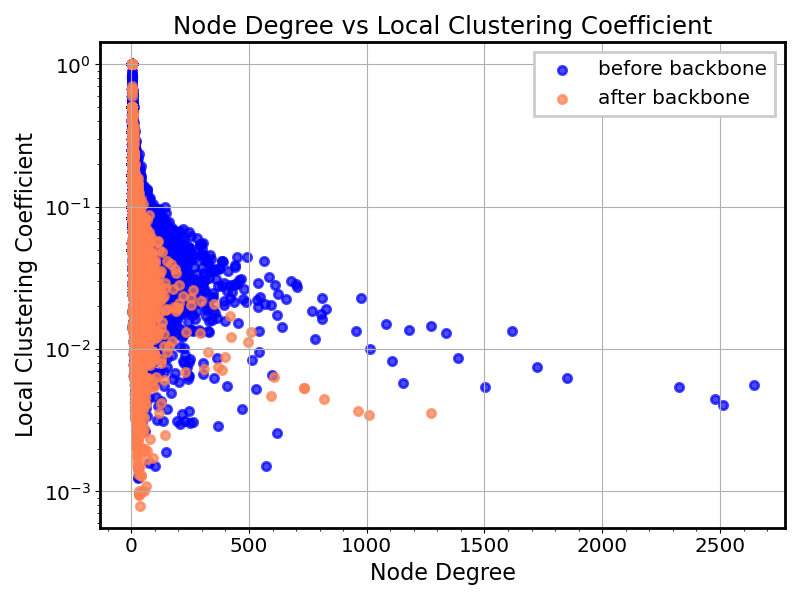
\includegraphics[width=\linewidth]{img/Node Degree vs Local Clustering Coefficient.png}
    \end{minipage}
   % \vspace{-10pt}
    \caption{Distribuzioni degree e local clustering coefficent prima e dopo il backboning\label{fig:backboning_dist}}
\end{figure}

\subsection{Inserimento opinioni} \label{sec:opinion}
L'obiettivo di questa sezione è assegnare un'opinione a ciascun utente basandosi sui loro upvotes e downvotes nei vari subreddit. Tuttavia, Reddit non fornisce accesso ai dati sui votanti dei post e commenti, rendendo impossibile assegnare direttamente le opinioni a chi ha espresso il voto. L'unico approccio possibile consiste nell'inferire le opinioni usando i voti ricevuti: un utente che ottiene molti upvote nei subreddit repubblicani è probabilmente pro-Trump, mentre uno che riceve molti upvote nei subreddit democratici è presumibilmente pro-Biden. Analogamente, numerosi downvote nei subreddit opposti suggeriscono che l'opinione espressa dall'utente non sia allineata con quella della comunità in cui ha postato.
Questo metodo è in grado di fornire solo un'approssimazione grossolana. Per i commenti, l'inferenza è meno immediata rispetto ai post: ad esempio, gli upvote su un commento critico vengono interpretati come supporto alla posizione del subreddit, anche se in realtà esprimono un'opinione opposta, poiché il metodo non distingue il contenuto ma solo i voti. Anche i post presentano questo problema, ma l'errore è attenuato dal maggior numero di visualizzazioni e da un pubblico tendenzialmente allineato con il subreddit. Per questo motivo, i voti sui commenti vengono ponderati meno rispetto a quelli sui post, assegnando un peso di 1 ai commenti e 1.5 ai post.
L'opinione viene rappresentata su una scala da 0 a 1, dove 1 indica supporto per Trump e 0 indica supporto per Biden. Il punteggio di ciascun utente viene calcolato in base ai voti ricevuti nei propri post e commenti: upvote nei subreddit repubblicani e downvote nei subreddit liberali aumentano il supporto a Trump, mentre upvote nei subreddit democratici e downvote nei subreddit repubblicani aumentano il supporto a Biden. L'opinione finale dell'utente i-esimo viene determinata mediante la seguente formula:
\begin{equation}
    \rm{opinione_i} = \frac{1}{2}  \left( \frac{\rm{supporto Trump_i} - \rm{supporto Biden_i}}{supporto  Totale_i} +1 \right)
\end{equation}

\begin{figure}[h]
    \centering
    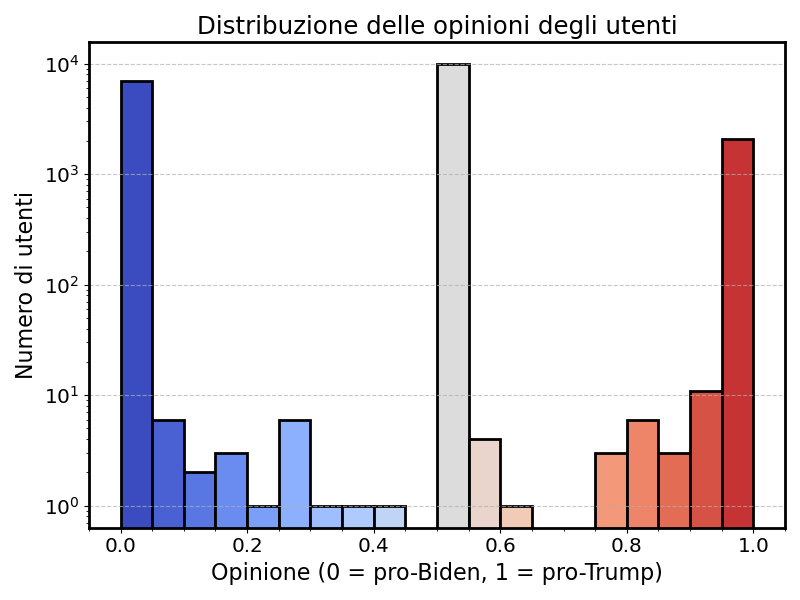
\includegraphics[width=\linewidth]{img/Distribuzione delle opinioni degli utenti.png}
    \caption{Distribuzioni opinione degli utenti} \label{fig:opinion_dist}
\end{figure}

In Figura \ref{fig:opinion_dist} è mostrata la distribuzione delle opinioni, evidenziando una polarizzazione verso gli estremi e un picco centrale che rappresenta gli utenti neutrali.
In Figura \ref{fig:gephi_graph} è rappresentato il grafo utilizzando \texttt{Gephi}. Confrontando la figura sopra, con i nodi colorati in base all'opinione assegnata, con la figura sotto, in cui gli archi sono colorati in base al subreddit di appartenenza, si osserva che la maggior parte dei nodi che vengono assegnati come neutrali appartengono al subreddit \textit{r/Conservative}, e quindi possono essere considerati come pro-Trump. 
Inoltre, in Figura \ref{fig:gephi_graph} sopra, si può vedere come le opinioni siano distribuite in modo ben distinto tra loro. Per quantificare questo fenomeno, si utilizza Newman's assortativity \cite{newman2003mixing}, che consente di calcolare l'homophily del grafo (la tendenza di un nodo a connettersi con nodi simili). I risultati, sia del grafo completo che nelle snapshot settimanali, sono riportati in Tabella \ref{tab:homophily}.

\begin{table}[ht]
    \centering
    \resizebox{\columnwidth}{!}{
    \begin{tabular}{|l||c||c|c|c|c|c|r|}
    \hline
     & Completo & \multicolumn{6}{c|}{Snapshot settimanali}\\
    \hline
    Homophily & 0.784 & 0.692 & 0.727 & 0.734 & 0.752 & 0.784 & 0.808 \\
    \hline
    \end{tabular}
    }
    \caption{Homophily rispetto all'opinione degli utenti}
    \label{tab:homophily}
\end{table}

\begin{figure}[h]
    \centering
    \begin{minipage}{0.48\textwidth}
        \centering
        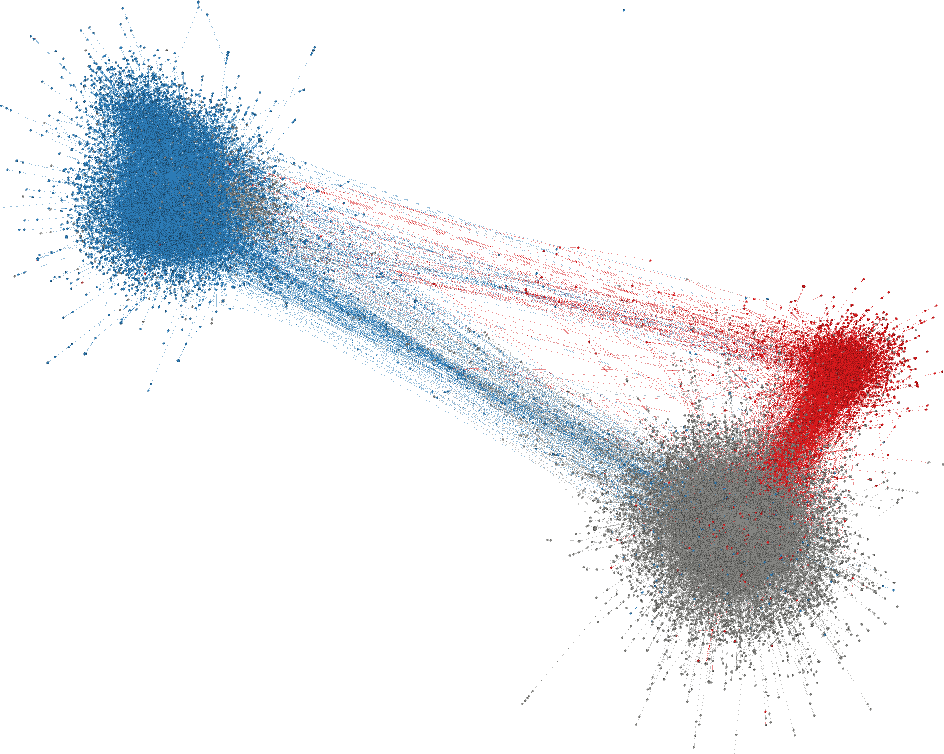
\includegraphics[width=\linewidth]{img/full_graph_backbone_opinion3.png}
    \end{minipage}
    \hfill
    \begin{minipage}{0.48\textwidth}
        \centering
        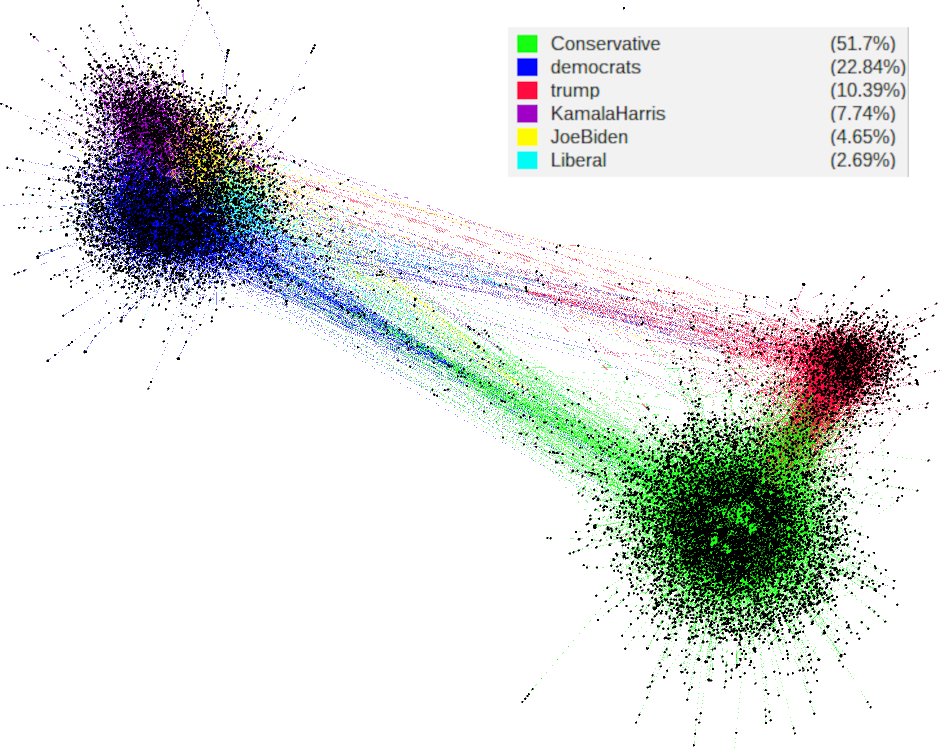
\includegraphics[width=\linewidth]{img/full_graph_backbone_subreddits5.png}
    \end{minipage}
   % \vspace{-10pt}
    \caption{Rappresentazione del grafo tramite Gephi. Sopra: il colore dei nodi rappresenta le opinioni assegnate; sotto: il colore degli archi rappresenta il subreddit di appartenenza. \label{fig:gephi_graph}}
\end{figure}

\section{Network Characterization}\label{sec:network_characterization}
Lo scopo di questa sezione è analizzare le caratteristiche del grafo. Inizialmente, verranno confrontate le proprietà di base con quelle di grafi sintetici; successivamente, verranno analizzati diversi tipi di centralità. 
Per semplicità, nell'analisi sono stati rimossi sia la direzione che il peso degli archi. Dopo la conversione, il numero di archi diminuisce a circa $\sim 66k$; perché coppie di archi, inizialmente distinti per ingresso e uscita tra due nodi, vengono unificate in un unico arco senza direzione.

Le caratteristiche principali del grafo reale e dei tre grafi sintetici analizzati (random, small world e scale-free) sono riportate in Tabella \ref{tab:graph_property}. In particolare, $N_c$ rappresenta il numero di componenti del grafo, $P_c$ indica la percentuale di nodi che appartengono alla componente principale, $\langle k \rangle$ corrisponde all'average degree, $C$ è il coefficiente di clustering globale, $\rho$ rappresenta la densità del grafo, mentre $\langle l \rangle$ è l'average shortest path. Tutti i grafi appartengono al regime supercritico essendo $\rho > 1/N \approx 0.05 \times 10^{-3}$ e $\rho < ln(N)/N \approx 0.52 \times 10^{-3}$.

Dai dati relativi al grafo reale emerge che sebbene vi siano numerose componenti, la componente principale comprende quasi tutti i nodi. Ciò suggerisce che le altre componenti siano frammenti costituiti da pochi nodi, il cui contributo al grafo complessivo è trascurabile. Per quanto riguarda gli altri parametri, è più efficace commentarli utilizzando appositi grafici di riferimento.

\begin{table}[ht]
    \centering
    \resizebox{\columnwidth}{!}{
        \begin{tabular}{l|c c c c}
        \hline
        \hline
         & Reale & Random & Small world & Scale-free\\
        \hline
        \hline
        $N_c$ & 216 & 19 & 1 & 1  \\
        \hline
        $P_c$ & 97.6\% & 99.9\% & 100\% & 100\%  \\
        \hline
        $\langle k \rangle$ & 7 & 7 & 6 & 6  \\
        \hline
        $C\; [10^{-2}]$ & 4.2 & 0.04 & 4.2  & 0.32 \\
        \hline
        $\rho \; [10^{-3}]$ & 0.37 & 0.37& 0.32 & 0.32 \\
        \hline
        $\langle l \rangle$ & 4.66 & 5.28 & 5.99 & 4.49  \\
        \hline
        \end{tabular}
    }
    \caption{Confronto tra il grafo reale e tre grafi sintetici.}
    \label{tab:graph_property}
\end{table}

\subsection{ Confronto con grafo random}
Il grafo random \cite{alfred1959publicationes} è stato creato a partire dal numero di nodi $N$ e dalla densità del grafo reale $\rho$. I valori dell'average degree risultano uguali, poiché $\langle k \rangle = \rho (N-1)$, dove $N$ e $\rho$ sono uguali tra i due grafi. Come atteso, il global clustering coefficient del random graph è molto minore rispetto a quello reale. Questo accade perché il grafo random non rispetta il principio di triadic closure (due nodi che condividono un vicino tendono a formare un legame). Infine, per quanto riguarda l'average shortest path, il valore nel grafo random risulta leggermente superiore rispetto a quello del grafo reale. Questo è dovuto al fatto che, nel regime random, si ha $\langle l \rangle \sim ln(N)/ln\langle k \rangle \approx 5.06$, mentre nel regime scale-free (che è più simile al grafo reale), la lunghezza media dei cammini passa per un punto critico, seguendo la relazione $\langle l \rangle \sim ln(N)/ln(ln(N)) \approx 4.31$. Un altro modo per giustificare la riduzione di $\langle l \rangle$ nel grafo reale è la presenza di hubs, che facilitano il raggiungimento di nodi distanti, contribuendo così a ridurre la lunghezza media del cammino.


\subsection{Confronto con grafo small world}
Per la generazione del grafo small world \cite{watts1998collective} sono necessari tre parametri: il numero di nodi, il grado medio e la probabilità di rewiring. Il numero di nodi viene mantenuto uguale a quello del grafo reale, mentre il grado medio viene impostato come $\langle k \rangle - 1$ rispetto a quello del grafo reale, in modo da ottenere un valore pari. Questo è necessario perché l'algoritmo parte da una configurazione iniziale in cui ogni nodo è connesso a un numero uguale di vicini a sinistra e a destra, garantendo così una struttura iniziale simmetrica e regolare prima dell'applicazione del rewiring. L'ultimo parametro, $p$, rappresenta la probabilità che un arco venga riscritto, collegando due nodi scelti casualmente. Quando $p=1$, il grafo risultante è random. Per determinare un valore ottimale di $p$, si dovrebbe analizzare l'andamento del coefficiente di clustering e della lunghezza media dei cammini al variare di $p$, con l'obiettivo di ottenere valori simili a quelli del grafo reale. In genere, ciò significa massimizzare il coefficiente di clustering e minimizzare la lunghezza media dei cammini. Tuttavia, poiché il calcolo di quest'ultima è computazionalmente costoso, scelgo un approccio più efficiente, variando $p$ in base al coefficiente di clustering e verificando successivamente se la lunghezza media dei cammini risulta comparabile a quella reale. Il valore selezionato è $p=0.59$, in quanto consente di ottenere un coefficiente di clustering pari a quello del grafo reale, mantenendo al contempo una bassa lunghezza media dei cammini. Come prima, il valore di $\langle l \rangle$ resta superiore a quello del grafo reale, in quanto il grafo si trova ancora nel regime random e segue la relazione $\langle l \rangle \sim ln(N)/ln\langle k \rangle \approx 5.50$. 

\subsection{Confronto con grafo scale-free}
Il grafo scale-free \cite{barabasi1999emergence} è stato creato utilizzando lo stesso numero di nodi $N$ del grafo reale e impostando il parametro $m\approx N/L$, dove $L$ è il numero di archi del grafo reale. Il parametro $m$ rappresenta il numero di collegamenti che ogni nuovo nodo crea al momento del suo ingresso nella rete. Visto che la degree distribution segue una legge di potenza, questo tipo di grafo consente la formazione di hubs, che riducono la lunghezza media dei cammini, portando a un valore di $\langle l \rangle$ simile a quello del grafo reale. D'altra parte, come il grafo random, il modello scale-free non rispetta il principio di triadic closure e, a differenza del grafo small-world, non è progettato per massimizzare il coefficiente di clustering. Di conseguenza, il valore di $C$ risulta inferiore rispetto a quello del grafo reale.

\begin{figure}[h]
    \centering
    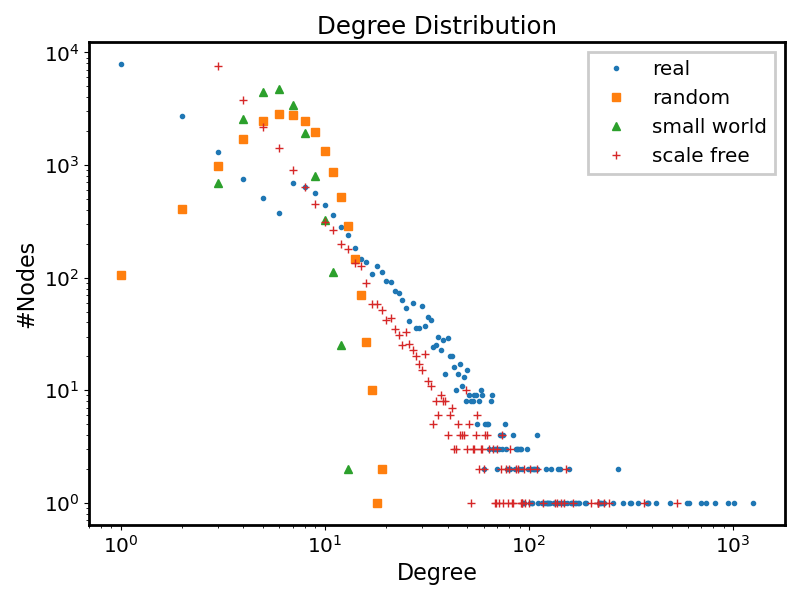
\includegraphics[width=\linewidth]{img/Degree_Distribution.png}
    \caption{Degree distribution del grafi sintetici rispetto al grafo reale} \label{fig:degree_dist}
\end{figure}

\subsection{Degree distribution}
In Figura \ref{fig:degree_dist} sono riportate le degree distribution dei vari grafi analizzati. I grafi random e small world seguono una distribuzione di tipo poissoniano, dove i degree dei nodi sono concentrati attorno al valore medio. Come discusso in precedenza, queste distribuzioni non permettono la formazione di hubs. Al contrario, il grafo scale-free segue una legge di potenza. Per vedere se questa distribuzione è compatibile con quella reale, è stato effettuato un fit utilizzando il metodo \textit{Kolmogorov–Smirnov} \cite{kolmogorov1933sulla}\cite{smirnov1948table} per determinare l'esponente $\gamma$. I risultati ottenuti sono $\gamma_{real} = 2.40 \pm 0.28$ e $\gamma_{sf} = 2.33 \pm 0.24$, dove l'errore è rappresentato dalla deviazione standard. I due parametri risultano compatibili, permettendo di concludere che il grafo scale-free ben rappresenta il grafo reale.

\begin{figure}[h]
    \centering
    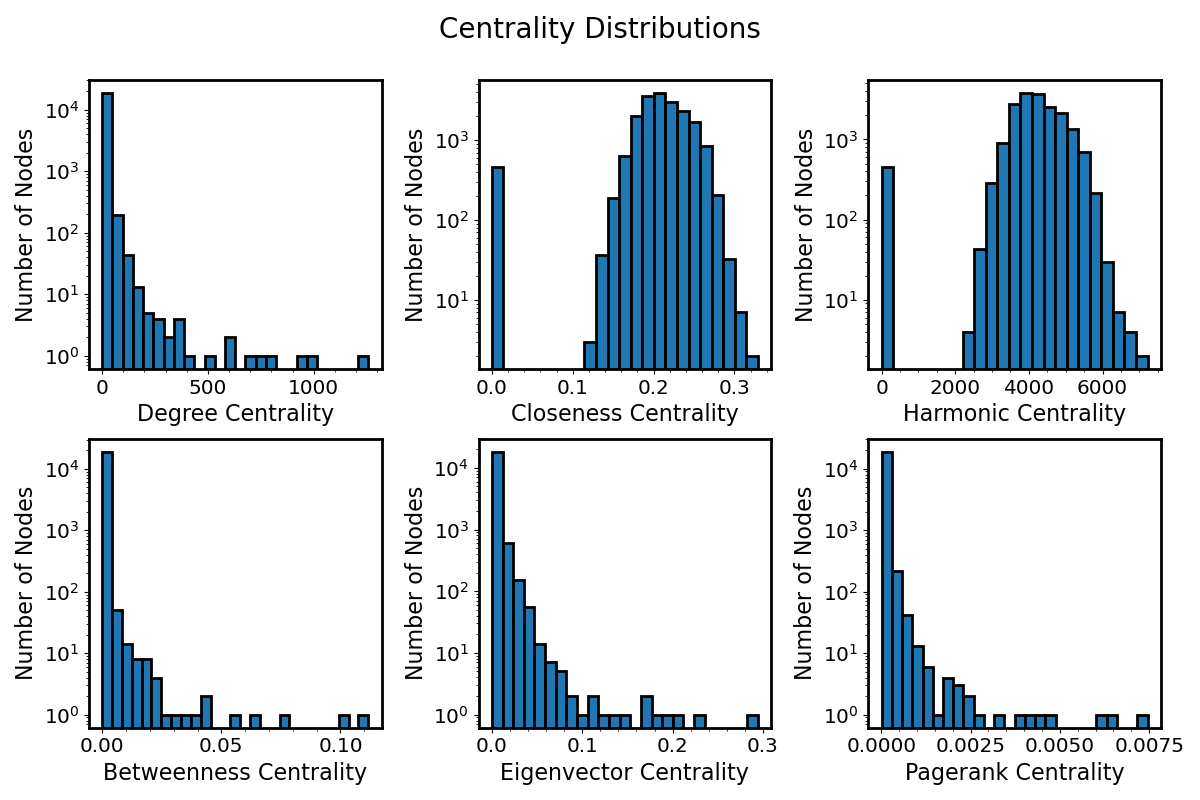
\includegraphics[width=\linewidth]{img/Centrality.png}
    \caption{Distribuzioni di diverse tipologie di centralità} \label{fig:centrality}
\end{figure}

\subsection{Centarlità}
In Figura \ref{fig:centrality} sono riportate le distribuzioni relative a sei tipologie di centralità: degree centrality, closeness centrality, harmonic centrality, betweenness centrality, eigenvector centrality e PageRank centrality.

La \textit{degree centrality} di un nodo misura il suo grado. La distribuzione evidenzia un'asimmetria verso sinistra, dovuta alla presenza di numerosi nodi a basso grado e di una minoranza di nodi ad alto grado (hubs). L'informazione di questo grafico è analoga a quella in Figura \ref{fig:degree_dist}.

Sia la \textit{closeness centrality} che la \textit{harmonic centrality} quantificano la vicinanza di un nodo rispetto a tutti gli altri del grafo. In particolare, la prima viene calcolata come l’inverso della media aritmetica degli shortest path che collegano il nodo a tutti gli altri, mentre la seconda si basa sulla media armonica di tali distanze. Il picco vicino a zero è dovuto ai nodi scollegati dalla componente principale. Quest'ultima è distribuita in modo simmetrico intorno al valore centrale, indicando che la maggior parte degli utenti ha un accesso simile agli altri nodi. Prendendo come riferimento la Figura \ref{fig:gephi_graph}, i valori al bordo o esterni al cluster corrispondono alla coda sinistra della distribuzione, mentre gli hubs si posizionano nella coda destra.

La \textit{betweenness centarlity} di un nodo misura il numero di shortest path che passano per quel nodo, indicando così il suo ruolo di ponte all'interno del grafo. La distribuzione mostra una forte asimmetria, con pochi nodi caratterizzati da un'elevata betweenness. In Figura \ref{fig:gephi_graph}, tali nodi corrispondono a quegli utenti che collegano i cluster nel grafo polarizzato, facilitando il flusso di informazioni tra opinioni differenti. Inoltre, la distribuzione permette di osservare una forte polarizzazione: la maggior parte dei nodi presenta infatti valori molto bassi di betweenness, suggerendo la formazione di echo chambers, dove gli utenti tendono a interagire esclusivamente con altri che condividono opinioni simili\footnote{È opportuno precisare che questa affermazione non è totalmente corretta, in quanto i dati sono stati estratti da subreddit già polarizzati; pertanto, il fenomeno delle echo chambers è stato in parte imposto durante la raccolta dei dati.}.

Infine, sia la \textit{eigenvector centrality }che la \textit{PageRank centrality} si basano sull'idea che un nodo acquisisca importanza se collegato a nodi anch'essi influenti.  Queste misure tengono conto non solo del numero di vicini, ma anche della loro centralità. Entrambe le distribuzioni risultano asimmetriche, con un numero ristretto di nodi ad alta centralità che corrispondono agli utenti più influenti, ovvero agli hubs.



\section{Open question: Diffusione opinioni} \label{sec:diffusion_opinion}
Nella simulazione della diffusione delle opinioni non è possibile impiegare il modello di algorithmic bias \cite{sirbu2019algorithmic}, poiché questo non considera né la direzionalità né il peso degli archi. Per tale motivo, nella classe \texttt{WeightedOpinionDiffusion} è stata implementata una variante del modello.

Per tenere conto della direzionalità degli archi, una volta selezionato un nodo, vengono considerate esclusivamente le interazioni in ingresso. Inoltre, l'aggiornamento dell'opinione interessa unicamente il nodo selezionato, in quanto la diffusione deve propagarsi lungo la direzione indicata dalle frecce.

Per quanto riguarda il peso degli archi, sono state apportate due modifiche. La prima consiste nel ridefinire la metrica delle distanze tra opinioni:
\begin{equation}
    d_i(j) = \frac{|o_i - o_j|}{w'_{ji}} 
\end{equation}
\begin{equation}
    \begin{cases}
        w'_{ji} = w_{ji} \hfill \text{se } \texttt{reduced\_weight=False} \\
        w'_{ji} = 1 + (w_{ji} - 1)/10 \hfill \text{   se } \texttt{reduced\_weight=True}
    \end{cases}
    \label{eq:reduced_weight}
\end{equation}
dove $o_i$ e $o_j$ rappresentano, rispettivamente, le opinioni degli utenti $i$ e $j$, e $w_{ji}$ è il peso dell'arco $j \rightarrow i$. Si noti che la distanza non è simmetrica, perché in generale $w_{ji} \neq w_{ij}$. Essendo $w_{ji} \geq 1$, il peso dell'arco incide in maniera significativa sulla distanza, rendendo trascurabili le probabilità di selezionare nodi con peso inferiore \footnote{La formula delle probabilità rimane analoga a quella del modello di algorithmic bias, cambia solo la metrica delle distanze.}. Ciò può rappresentare un problema in presenza di grafi polarizzati, in cui il peso degli archi interni ai cluster è solitamente superiore rispetto a quello degli archi che collegano i cluster, confinando così la diffusione all'interno dei singoli cluster. Per attenuare tale fenomeno è stato introdotto il parametro \texttt{reduced\_weight}, che, se impostato su \texttt{True}, modifica il valore del peso come indicato nell'Equazione \ref{eq:reduced_weight} (ad esempio: $w_{ji} = 1 \rightarrow w'_{ji} = 1, \; w_{ji} = 2 \rightarrow w'_{ji} = 1.1,\; w_{ji} = 3 \rightarrow w'_{ji} = 1.2$, ...).

La seconda modifica riguarda l'aggiornamento dell'opinione, che avviene mediante una media pesata:
\begin{equation}
    o'_i = \frac{o_i + w'_{ji}o_j}{1+w'_{ji}}
\end{equation}
dove $o'_i$ rappresenta l'opinione aggiornata dell'utente $i$. Come già accennato, l'opinione dell'utente $j$ non viene modificata. Anche in questa formula il peso viene ridotto se il parametro  \texttt{reduced\_ weight} è impostato su \texttt{True}.

Il modello è gestito da una seconda classe, \texttt{OpinionDiffusion Simulator}, che consente di simulare il processo di diffusione delle opinioni dopo aver configurato i seguenti parametri:
\begin{itemize}
    \item \textbf{iterations}: numero di iterazioni;
    \item \textbf{epsilon} e \textbf{bias}: come nel modello di  algotitmic bias, rappresentano rispettivamente l'open-mindedness e il bias;
    \item \textbf{reduced\_weight}: riduce l'influenza del peso secondo l'equazione \ref{eq:reduced_weight};
    \item \textbf{random\_opinion}: imposta l'inizializzazione casuale delle opinioni degli utenti.
\end{itemize}

Inoltre, la classe include funzioni per la creazione di tre differenti grafici:
\begin{enumerate}
    \item Il primo mostra la distribuzione delle opinioni al termine del processo.
    \item Il secondo suddivide le opinioni in tre categorie ("pro-Trump", "pro-Biden" e "neutral") e consente di osservare l'evoluzione del numero di utenti appartenenti a ciascuna categoria.
    \item Il terzo grafico visualizza l'andamento dell'opinione di ciascun utente nel tempo.
\end{enumerate}

\begin{figure}[h]
    \centering
    \begin{minipage}{0.48\textwidth}
        \centering
        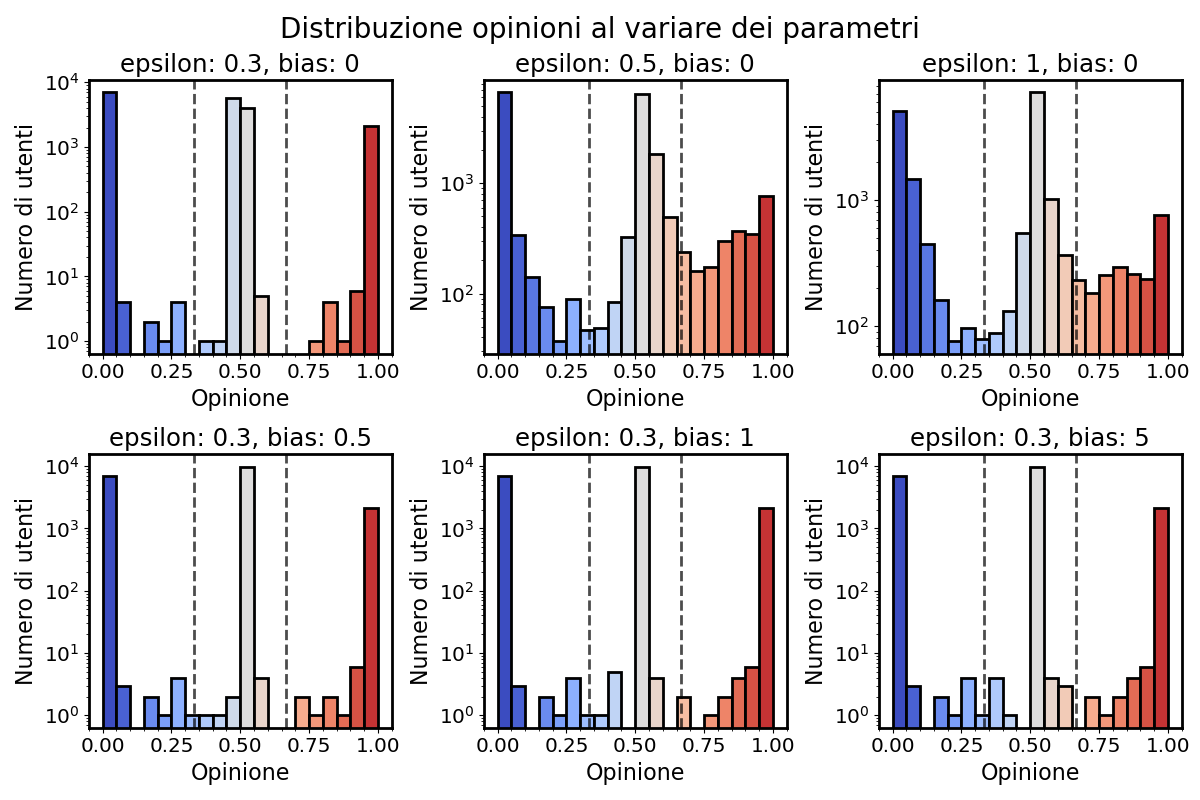
\includegraphics[width=\linewidth]{img/Distribuzione opinioni al variare dei parametri.png}
    \end{minipage}
    \hfill
    \begin{minipage}{0.48\textwidth}
        \centering
        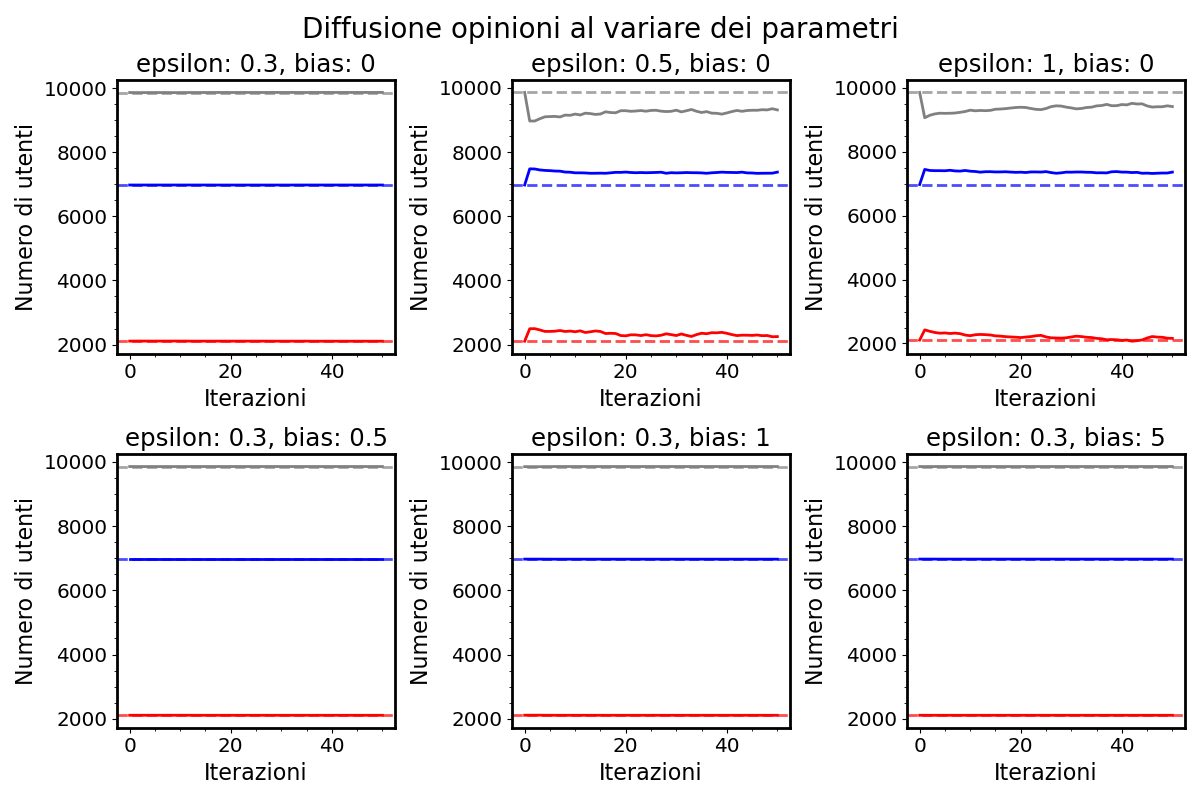
\includegraphics[width=\linewidth]{img/Diffusione opinioni al variare dei parametri.png}
    \end{minipage}
   % \vspace{-10pt}
    \caption{Risultati della diffusione delle opinioni. Sopra: la distribuzione delle opinioni alla fine del processo; sotto: la variazione degli utenti nelle tre categorie di opinione. \label{fig:opinion_diffusion}}
\end{figure}

\begin{figure}[h]
    \centering
    \begin{minipage}{0.48\textwidth}
        \centering
        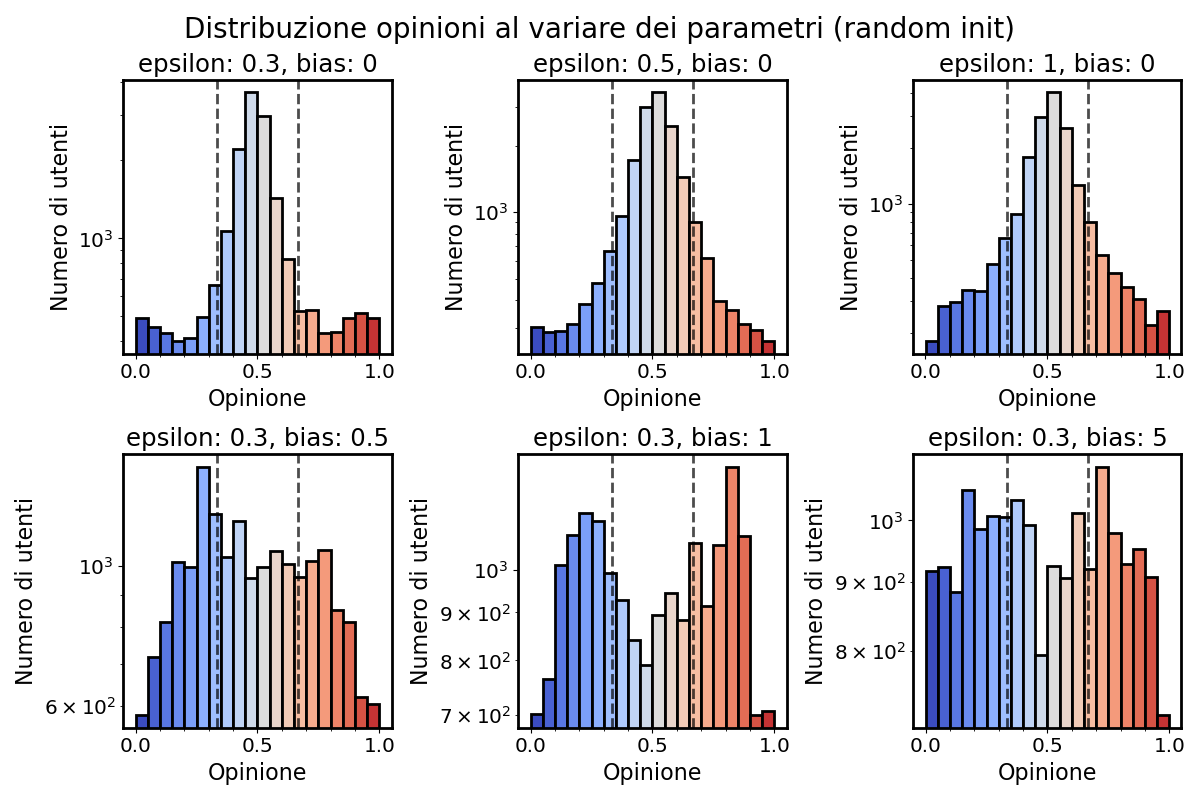
\includegraphics[width=\linewidth]{img/Distribuzione opinioni al variare dei parametri (random init).png}
    \end{minipage}
    \hfill
    \begin{minipage}{0.48\textwidth}
        \centering
        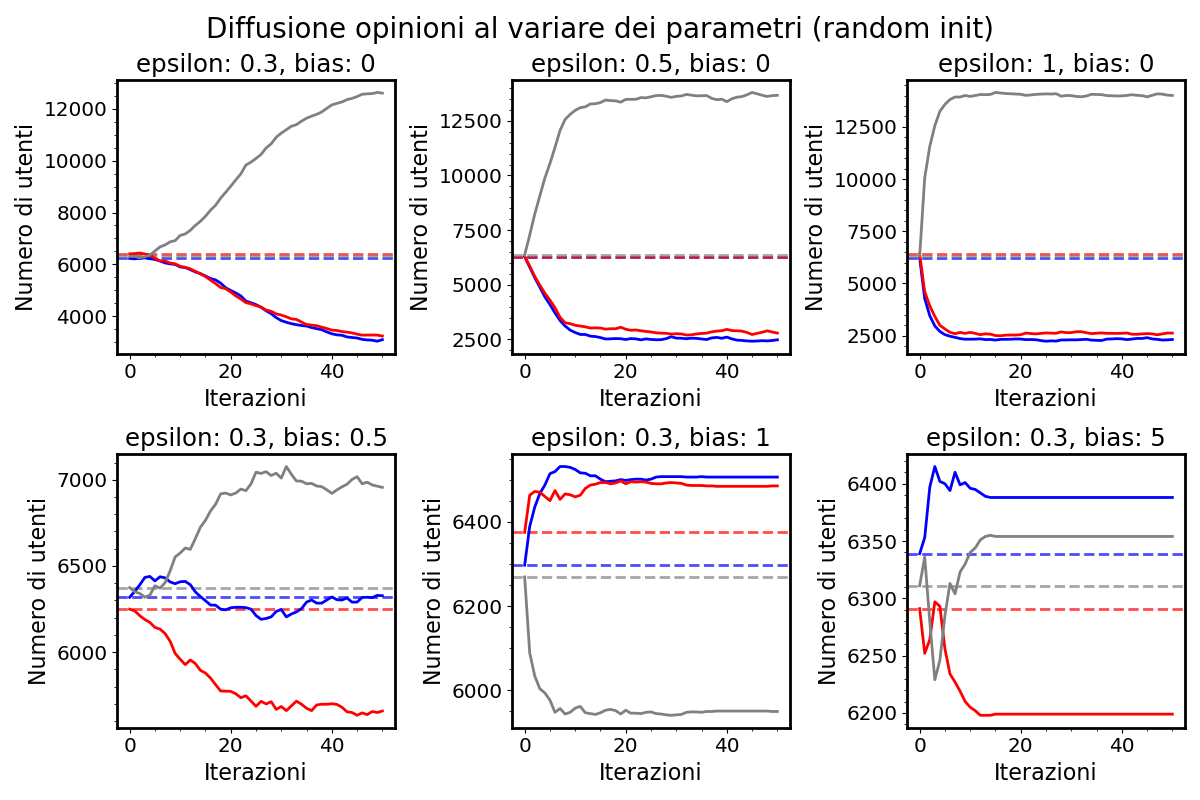
\includegraphics[width=\linewidth]{img/Diffusione opinioni al variare dei parametri (random init).png}
    \end{minipage}
   % \vspace{-10pt}
    \caption{Risultati della diffusione delle opinioni con inizializzazione random. Sopra: la distribuzione delle opinioni alla fine del processo; sotto: la variazione degli utenti nelle tre categorie di opinione. \label{fig:opinion_diffusion_random}}
\end{figure}

Nelle Figure \ref{fig:opinion_diffusion} e \ref{fig:opinion_diffusion_random} vengono illustrate le prime due tipologie di grafici ottenuti variando i parametri \texttt{epsilon} e \texttt{bias}. In particolare, nella prima figura le opinioni sono inizializzate con i valori calcolati in Sezione \ref{sec:opinion}, mentre nella seconda l'inizializzazione è casuale. Nella distribuzione delle opinioni (figura sopra) le linee tratteggiate verticali rappresentano la divisione tra le tre categorie illustrate nella diffusione (figura sotto). Invece, nella diffusione delle opinioni, le linee tratteggiate orizzontali rappresentano i valori iniziali delle categorie prima della diffusione.

Nel caso dell'inizializzazione manuale (Figura \ref{fig:opinion_diffusion}) si osserva che l'opinione tende a rimanere confinata all'interno dei cluster, nonostante la riduzione dei pesi. È presente solo una piccola variazione all'aumentare del parametro \texttt{epsilon} che aumenta il range in cui due opinioni possono interagire. È da notare che \texttt{epsilon} viene applicato alle distanze: quindi, anche se la differenza tra le opinioni supera questo valore, l'interazione è comunque possibile se il peso dell'arco è sufficientemente grande.
Nel caso dell'inizializzazione casuale (Figura \ref{fig:opinion_diffusion_random}) emergono invece i tipici effetti della diffusione delle opinioni: una convergenza sempre più rapida verso il valore centrale con l'aumentare di \texttt{epsilon} (come evidenziato nelle prime tre figure) e la comparsa di una polarizzazione con l'introduzione del bias (particolarmente evidente nella quinta figura, dove $\texttt{epsilon}=0.3$ e $\texttt{bias}=1$).

\begin{figure}[h]
    \centering
    \begin{minipage}{0.48\textwidth}
        \centering
        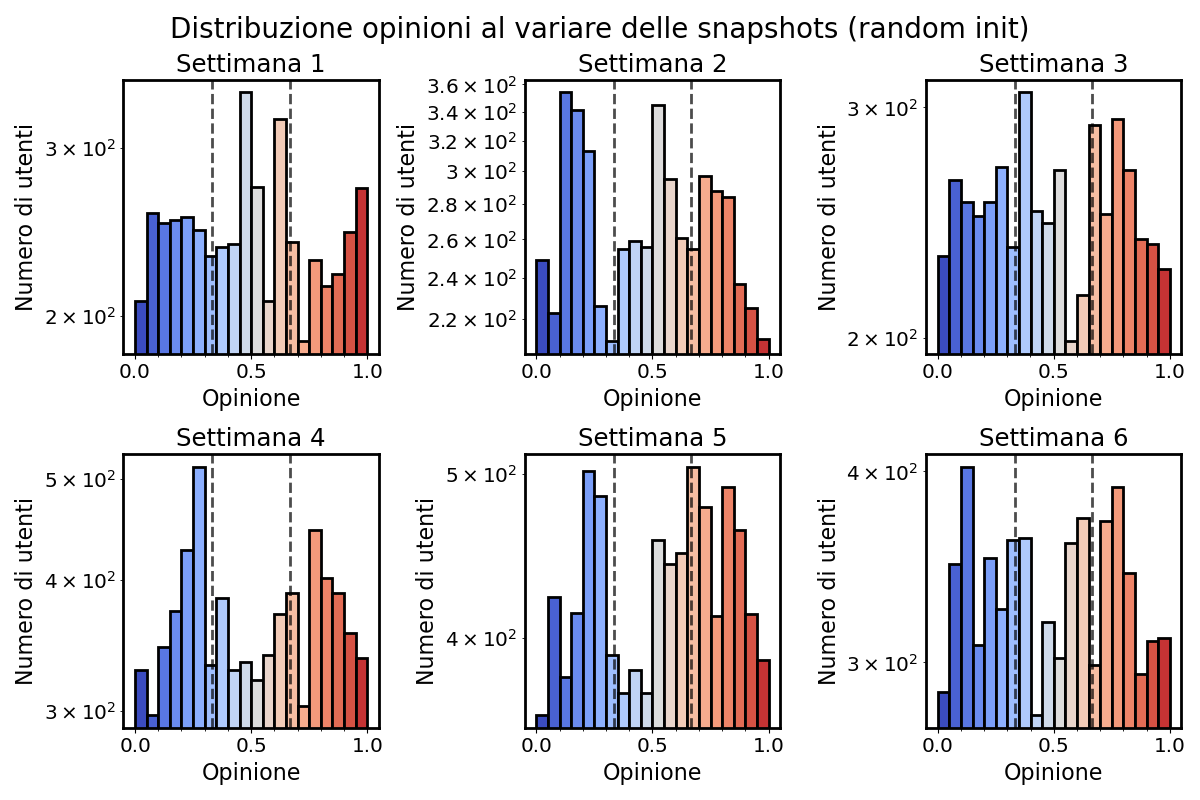
\includegraphics[width=\linewidth]{img/Distribuzione opinioni al variare delle snapshots (random init).png}
    \end{minipage}
    \hfill
    \begin{minipage}{0.48\textwidth}
        \centering
        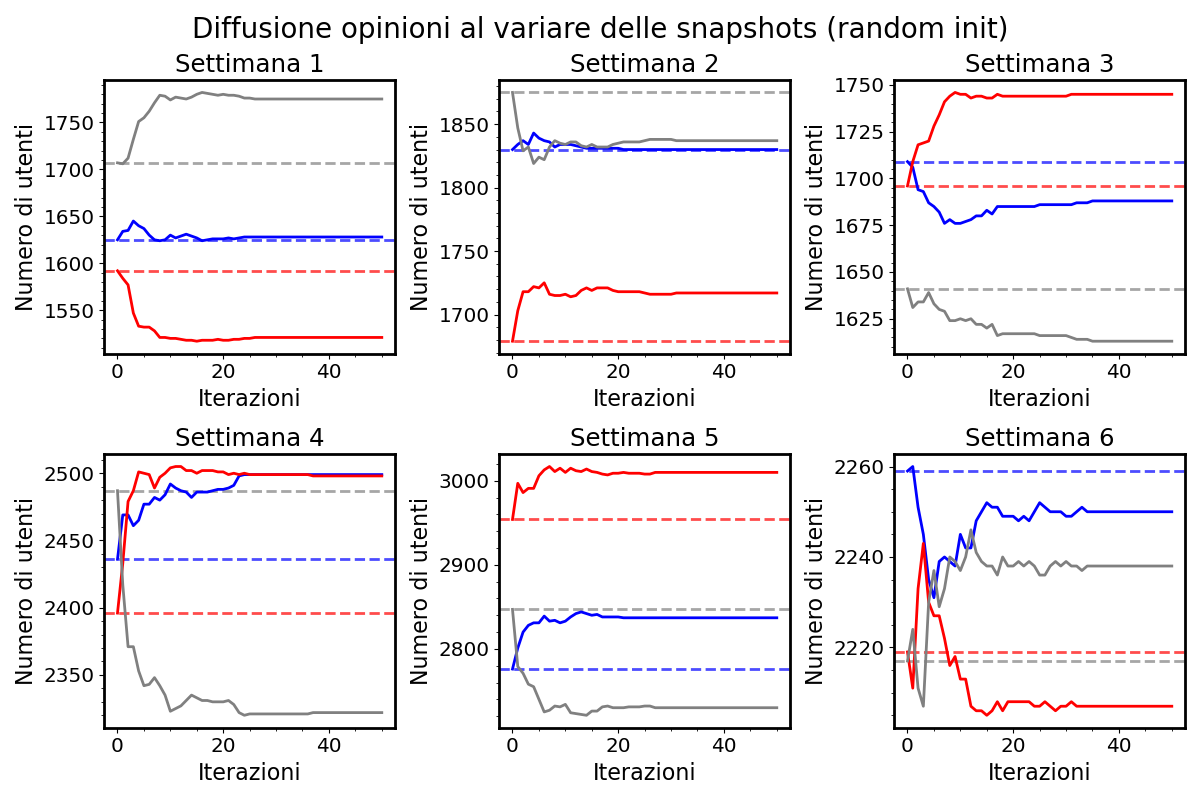
\includegraphics[width=\linewidth]{img/Diffusione opinioni al variare delle snapshots (random init).png}
    \end{minipage}
   % \vspace{-10pt}
    \caption{Risultati della diffusione delle opinioni negli snapshot. Sopra: la distribuzione delle opinioni alla fine del processo; sotto: la variazione degli utenti nelle tre categorie di opinione. \label{fig:opinion_diffusion_snapshot}}
\end{figure}

In Figura \ref{fig:opinion_diffusion_snapshot} mostra la diffusione delle opinioni in ciascuno snapshot, con parametri $\texttt{epsilon}=0.3$, $\texttt{bias}=1$ e \texttt{random\_ opinion}=\texttt{True}, scelti in base al precedente risultato che presentava la maggiore polarizzazione. I grafici non evidenziano particolari informazioni significative; sarebbe stato interessante osservare un aumento più marcato della polarizzazione nelle ultime tre settimane. Tuttavia, si nota un leggero aumento della polarizzazione nelle settimane 3 e 4.

\section{Open question: Evoluzione community} \label{sec:evoluzione_community}
Come descritto nella Sezione \ref{sec:introduction}, il grafo è stato suddiviso in sei snapshot, ognuno corrispondente a una settimana, ed è stata rimossa la direzionalità degli archi. Le componenti principali degli snapshot includono tra il $92,7\%$ e il $95,4\%$ dei nodi; pertanto, è possibile escludere i nodi rimanenti senza perdere informazioni significative, evitando così la formazione di un eccesso di community dovuto alla presenza di piccoli gruppi di nodi isolati.

Il modello di dynamic community discovery adottato è l'instant optimal \cite{greene2010tracking}, che utilizza il metodo Louvain \cite{blondel2008fast} per identificare le community nei vari snapshot e il Jaccard score per effettuare il matching tra di esse. L'analisi seguente è gestita dalla classe \texttt{CommunityEvolutionAnalysis}, che sfrutta la libreria \texttt{CDlib} \cite{rossetti2019cdlib}. Tale classe permette sia di generare grafici per la visualizzazione, sia di eseguire l'analisi dell'evoluzione delle community con un numero prefissato di ripetizioni.

\begin{figure}[h]
    \centering
    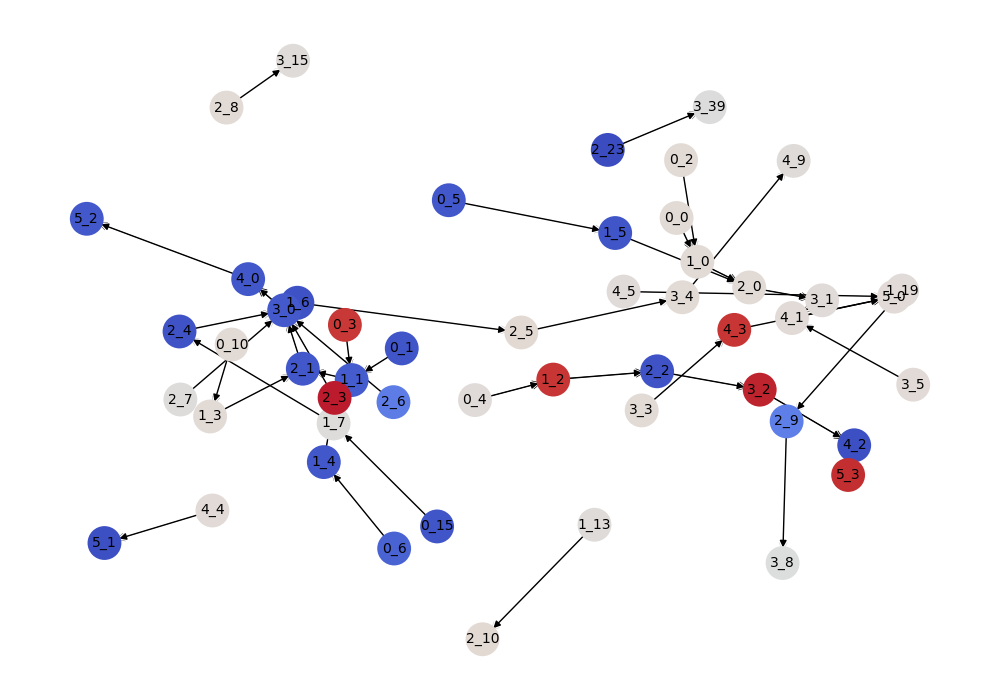
\includegraphics[width=\linewidth]{img/Evoluzione_community.png}
    \caption{Evoluzione delle community} \label{fig:community}
\end{figure}

In Figura \ref{fig:community} è illustrato il grafo che rappresenta l'evoluzione delle community. Per semplificarne la visualizzazione è stato applicato un filtro, mantenendo solo i match con un Jaccard score superiore al 78° percentile. Le etichette dei nodi sono composte da due numeri: il primo indica la snapshot, il secondo la community, mentre il colore dei nodi rappresenta l'opinione media degli utenti all'interno di ciascuna community. Si evidenzia come alcune community modifichino la propria opinione nel corso delle settimane.

\begin{figure}[h]
    \centering
    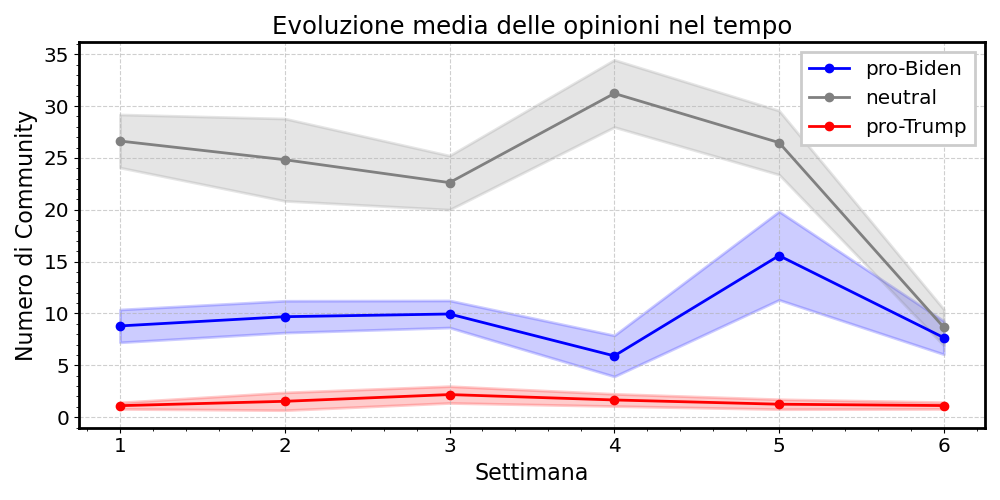
\includegraphics[width=\linewidth]{img/Evoluzione_opinioni_medie.png}
    \caption{Evoluzione del numero di community nelle tre categorie} \label{fig:num_community}
\end{figure}

In Figura \ref{fig:num_community} è mostrata l'evoluzione del numero di community, suddivise nelle tre categorie definite in Sezione \ref{sec:diffusion_opinion}. Considerando la natura non deterministica del metodo di Louvain, l'algoritmo è stato eseguito 100 volte, calcolando per ciascuna ripetizione la media e la deviazione standard (ques'ultima rappresentata nella figura come una banda). Nella quarta settimana, iniziata con l'attentato di Trump, si osserva un picco positivo per i neutrali (che assumeremo pro-Trump, essendo conservatori) e un picco negativo per i pro-Biden. Al contrario, nella quinta settimana, il cui secondo giorno coincide con la candidatura di Harris, si registra un aumento dei pro-Biden, mentre i neutrali diminuiscono.

\subsection{Validazione}
Per valutare i risultati dell'analisi è necessario creare un null model, ottenuto tramite sequence shuffling, ovvero mescolando l'ordine temporale degli snapshot. Sono state considerate tutte le permutazioni possibili, ad eccezione dell'ordine temporale originale ($6! - 1 = 719$). In Figura \ref{fig:null_model} sono mostrati i risultati del null model, con media e deviazione standard calcolate sulle 719 combinazioni. Si osserva una diminuzione del numero di community all'ultimo punto, dovuta al fatto che vengono salvate solo le community con matching: essendo l'ultimo snapshot privo di un successivo, non viene effettuato il matching.

\begin{figure}[h]
    \centering
    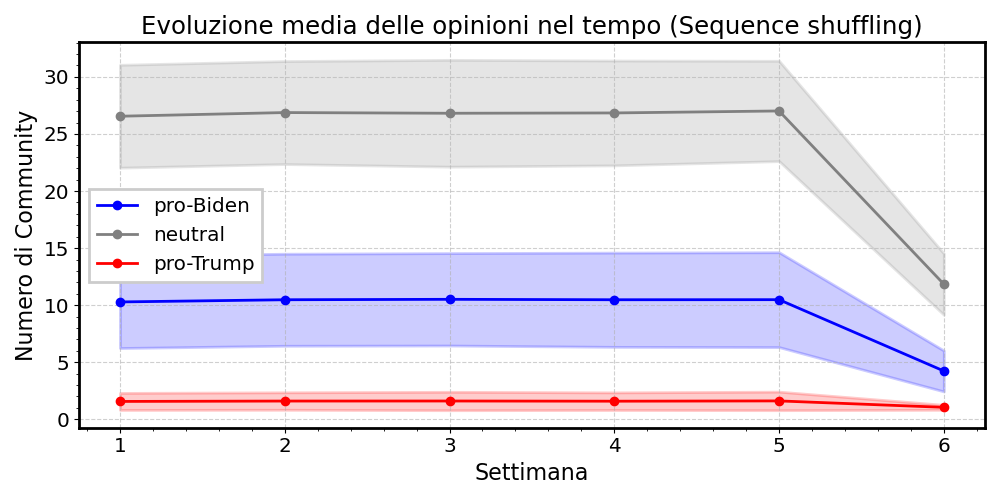
\includegraphics[width=\linewidth]{img/Sequence_shuffling.png}
    \caption{Evoluzione del numero di community per il null model} \label{fig:null_model}
\end{figure}

Per la valutazione si utilizza lo z-test, ma prima di applicarlo è necessario verificare che le distribuzioni dei campioni seguano una distribuzione gaussiana. In Figura \ref{fig:samples_dist} sono riportate le 18 distribuzioni (una per ciascun punto del grafico in Figura \ref{fig:num_community}), con il fit di una gaussiana sovrapposto. Il fit è stato ottenuto mediante il metodo del minimo $\chi^2$. Poiché per eseguire il fit è necessario stimare l'errore associato a ciascun bin dell'istogramma, e considerando che i bins rappresentano conteggi che seguono una distribuzione di Poisson, l'errore su ciascun bin è stato assunto pari alla radice quadrata del valore stesso.

\begin{figure}[h]
    \centering
    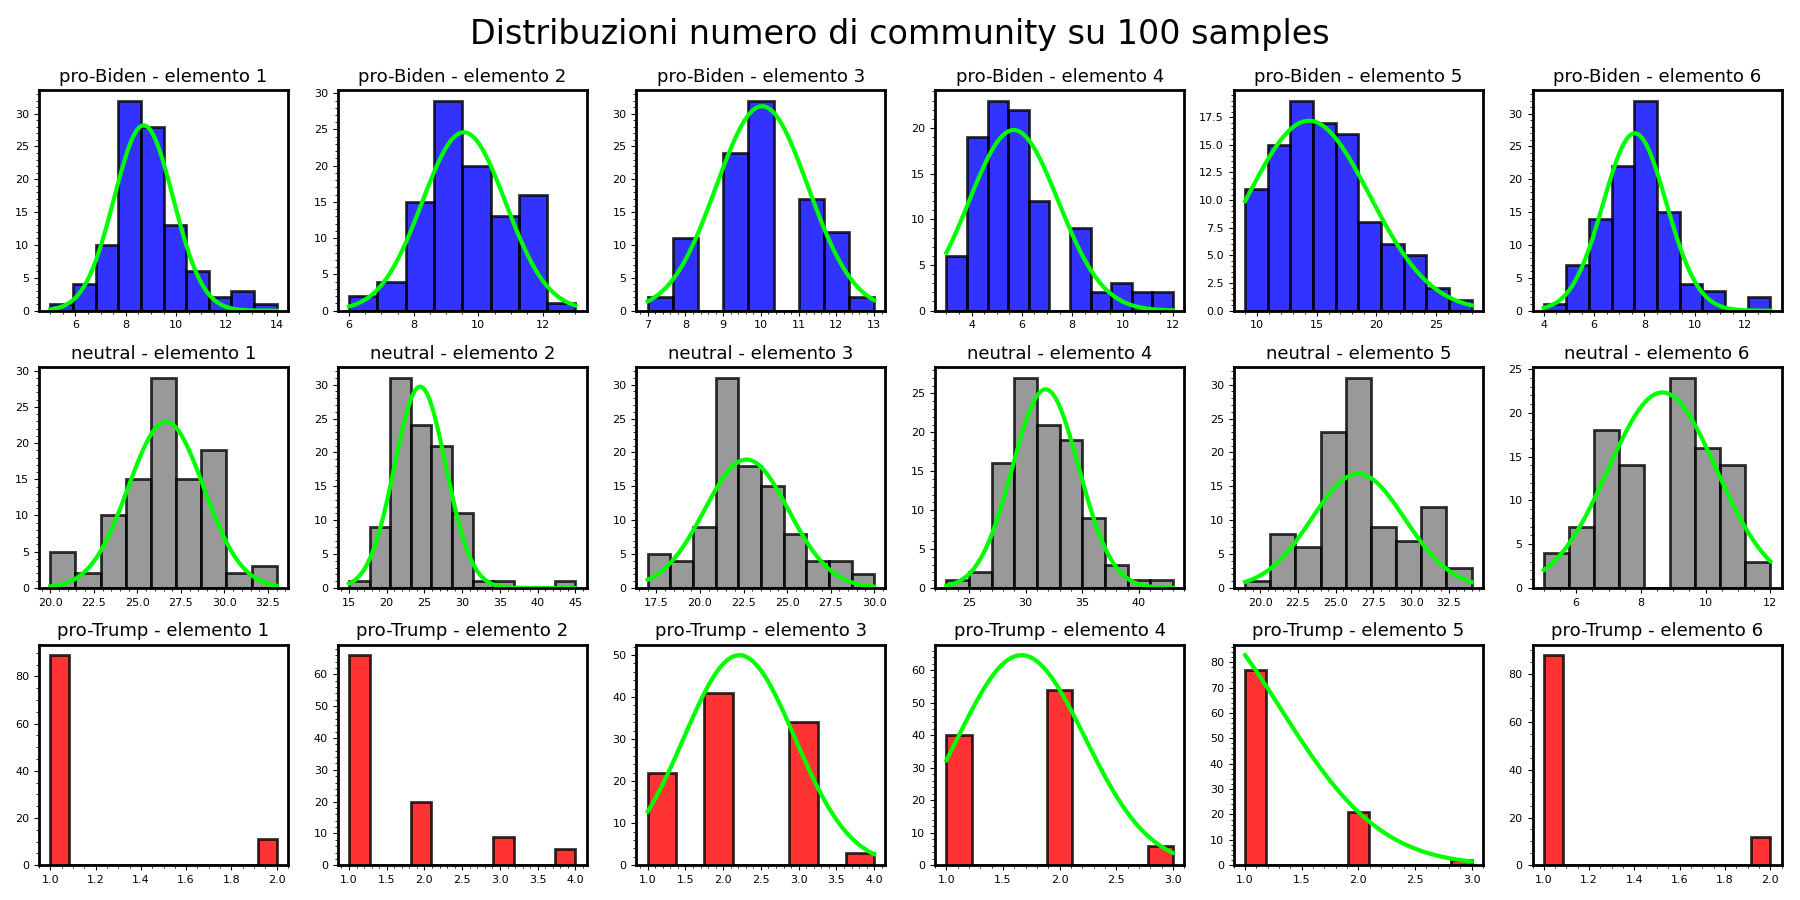
\includegraphics[width=\linewidth]{img/Distribuzione_community_samples.png}
    \caption{Distribuzione del numero community per i campioni} \label{fig:samples_dist}
\end{figure}


\begin{table}[ht]
    \centering
        \begin{tabular}{l|c c c c c c}
        \hline
        \hline
         $\chi^2/\nu$ & 1 & 2 & 3 & 4 & 5 & 6 \\
        \hline
        \hline
        pro-Biden & 1.1 & 1.9 & 0.8 & 1.6 & 0.2 & 1.0  \\
        \hline
        neutral & 2.3 & 1.2 & 1.8 & 0.9 & 3.8 & 1.2  \\
        \hline
        pro-Trump & - & - & 4 & nan & nan & -  \\
        \hline
        \end{tabular}
    \caption{Risultati fit con gaussiana}
    \label{tab:gauss_fit}
\end{table}

In Tabella \ref{tab:gauss_fit} sono riportati i risultati del fit espressi come $\chi^2/\nu$, dove $\nu$ rappresenta i gradi di libertà (calcolati come il numero di bin meno i parametri della gaussiana). Un valore di $\chi^2/\nu \approx 1$ indica un buon fit, mentre $\chi^2/\nu \gg 1$ segnala che la distribuzione non segue una gaussiana.

Nel caso dei pro-Trump, l'algoritmo non è riuscito a eseguire il fit per le distribuzioni delle settimane 1, 2 e 6. Per le settimane 4 e 5, essendo tre i parametri della gaussiana, si ottiene $\nu = 0$. I risultati indicano che le distribuzioni pro-Trump non seguono una distribuzione gaussiana, rendendo lo z-test non applicabile per questa categoria; in questo caso, sarebbe più appropriato utilizzare un t-test. Possiamo invece assumere che le distribuzioni pro-Biden e neutrali siano gaussiane e procedere con lo z-test per queste due categorie.

\begin{figure}[h]
    \centering
    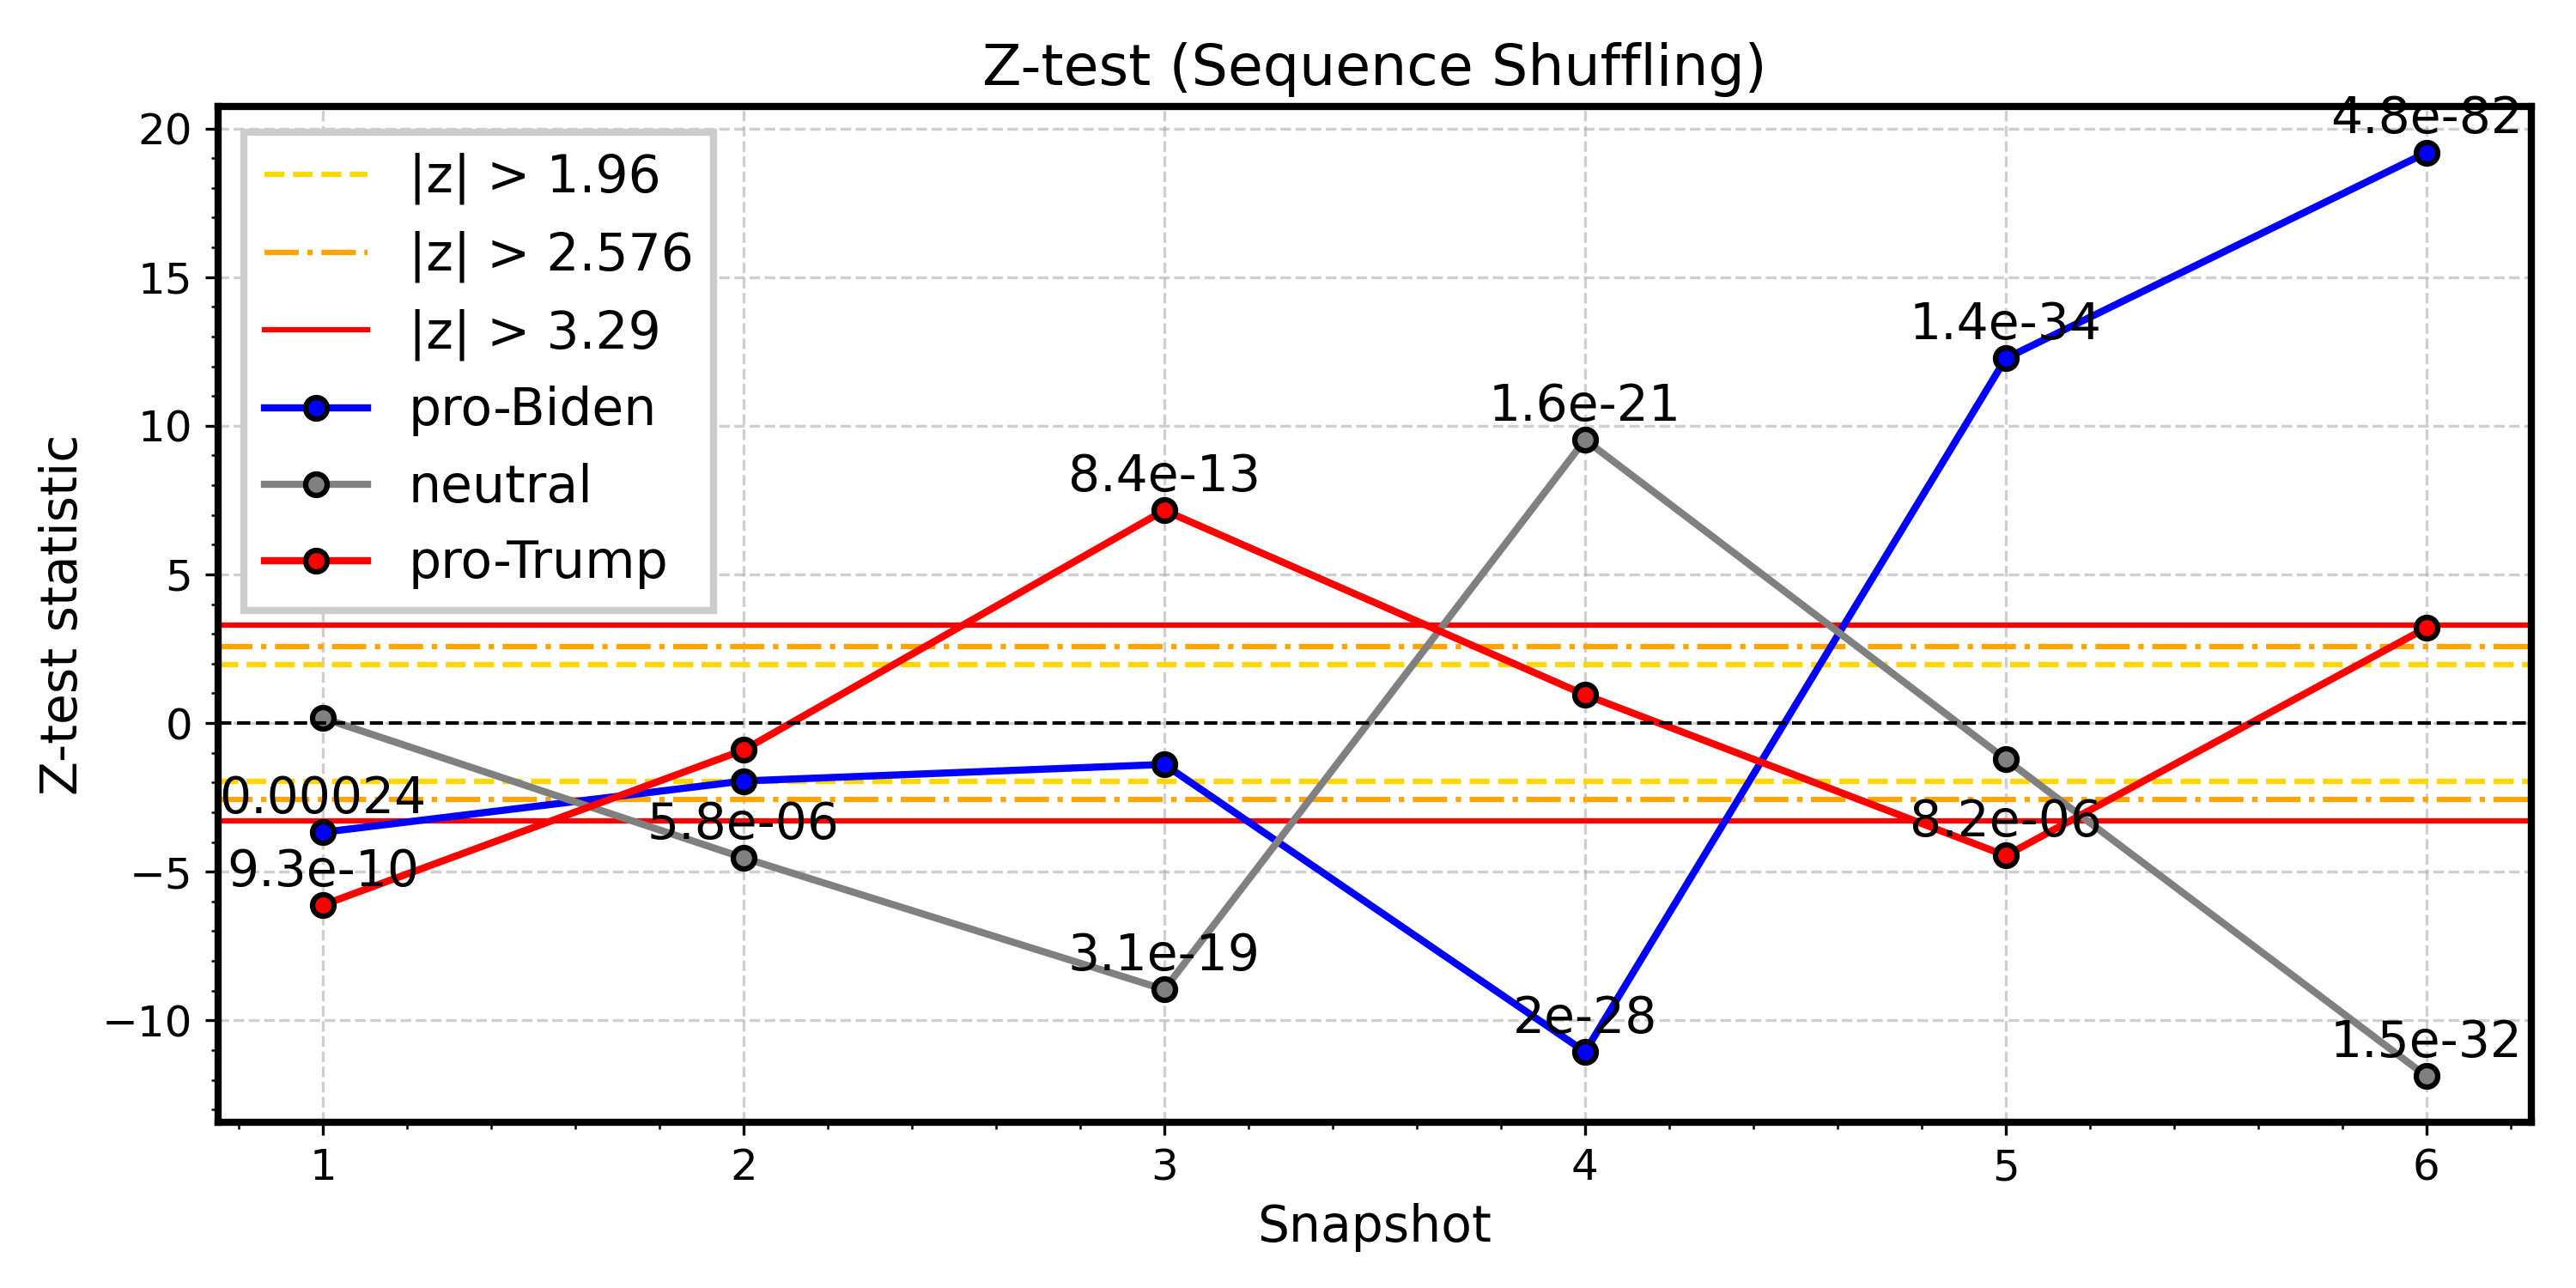
\includegraphics[width=\linewidth]{img/Ztest_Sequence_shuffling.png}
    \caption{z-test dell'evoluzione del  numero di community} \label{fig:z-test}
\end{figure}

In Figura \ref{fig:z-test} sono riportati i risultati dello z-test per ciascuna distribuzione. La formula utilizzata è:
\begin{equation}
    z_{test} = \frac{\mu_{obs} - \mu_{H0}}{\sigma_{H0}/\sqrt{N_{obs}}}
\end{equation}
dove $\mu_{obs}$ e $\mu_{H0}$ rappresentano rispettivamente la media dei valori osservati (Figura \ref{fig:num_community}) e la media del null model (Figura \ref{fig:null_model}), $\sigma_{H0}$ è la deviazione standard del null model, mentre $N_{obs}$ indica il numero di valori osservati (100 ripetizioni).

Nel grafico sono evidenziate le fasce corrispondenti a $|z| > 1.96$ (p-value $< 0.05$), $|z| > 2.567$ (p-value $< 0.01$) e $|z| > 3.29$ (p-value $< 0.001$). Inoltre, sono riportati i valori di p-value per i risultati più significativi che superano la soglia esterna.

Si può concludere che i picchi nella terza e quarta settimana individuati in figura \ref{fig:num_community} sono significativi.  Tale andamento suggerisce un incremento della discussione a favore di Trump in seguito al suo attentato, seguito da un sostegno maggiore a Harris in concomitanza con la sua candidatura. Inoltre, si osserva come la candidatura di Harris abbia contribuito, almeno nel breve termine, ad attenuare l'effetto dell'attentato.

\section{Commenti finali}\label{sec:conclusioni}
L'analisi presenta quattro criticità:
\begin{enumerate}
    \item I dati raccolti non sono sufficienti per trarre conclusioni sulle opinioni degli utenti, in particolare servirebbero anche fonti neutrali.
    \item Il periodo considerato è ristretto e permette di osservare solo effetti a breve termine. Sarebbe preferibile estendere l'analisi fino al periodo elettorale per avere una visione più completa delle reazioni.
    \item L'analisi risulta fortemente influenzata dalla stima delle opinioni, la quale è stata effettuata in modo grossolano. Una possibile modifica potrebbe essere, dopo aver selezionato i parametri opportuni, quella di sfruttare i risultati della Sezione \ref{sec:diffusion_opinion} per studiare l'evoluzione delle community nelle tre categorie
    \item L'incremento del numero di community non dipende esclusivamente dal passaggio tra categorie, ma può anche essere il risultato della frammentazione di community all'interno della stessa categoria. Per rendere più esplicita l'informazione, potrebbe essere utile concentrarsi esclusivamente sulle transizioni tra categorie.
\end{enumerate}


% The next two lines define the bibliography style to be used, and the bibliography file.
\bibliographystyle{ACM-Reference-Format}
\bibliography{biblio}

\end{document}

